\chapter{Schaltpl�ne}

%\begin{figure}[ht]
%	\centering
%		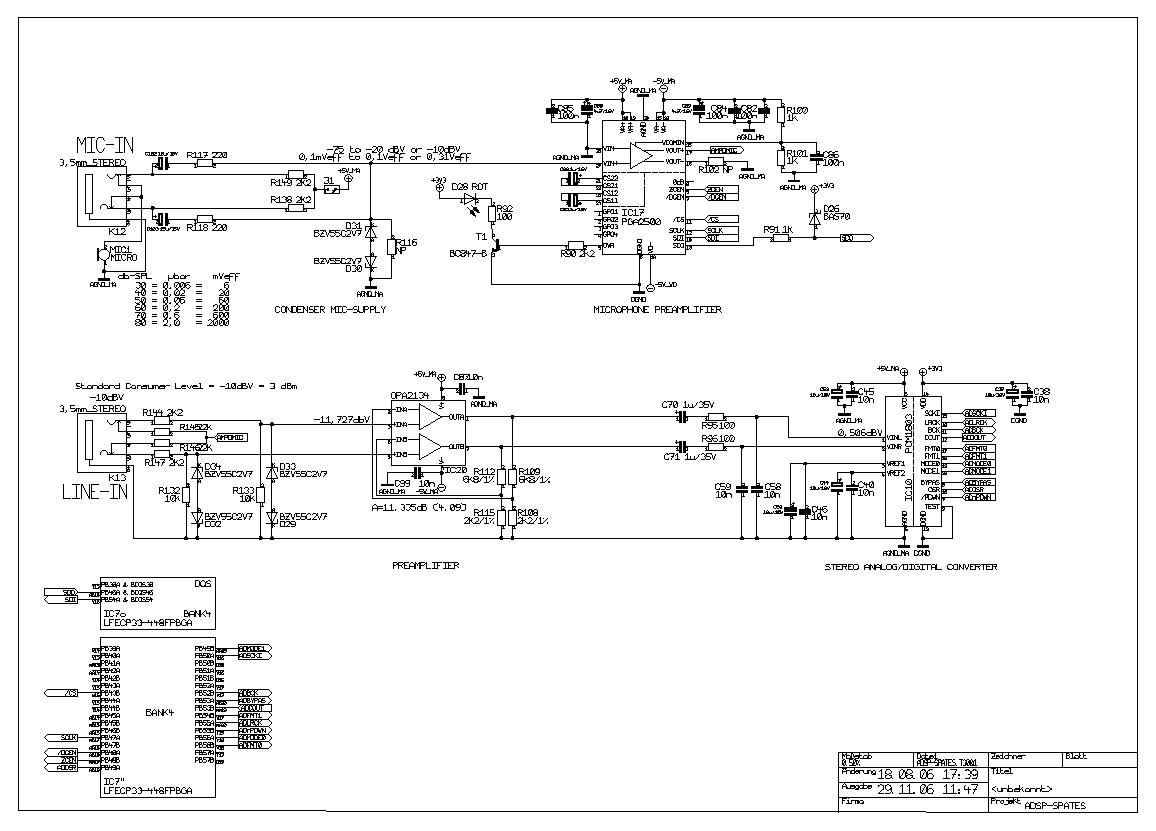
\includegraphics[angle=90,width=1.00\textwidth]{schematics/ADSP-SPATES_1}
%	\label{fig:schematic1}
%\end{figure}
%
%\begin{figure}[ht]
%	\centering
%		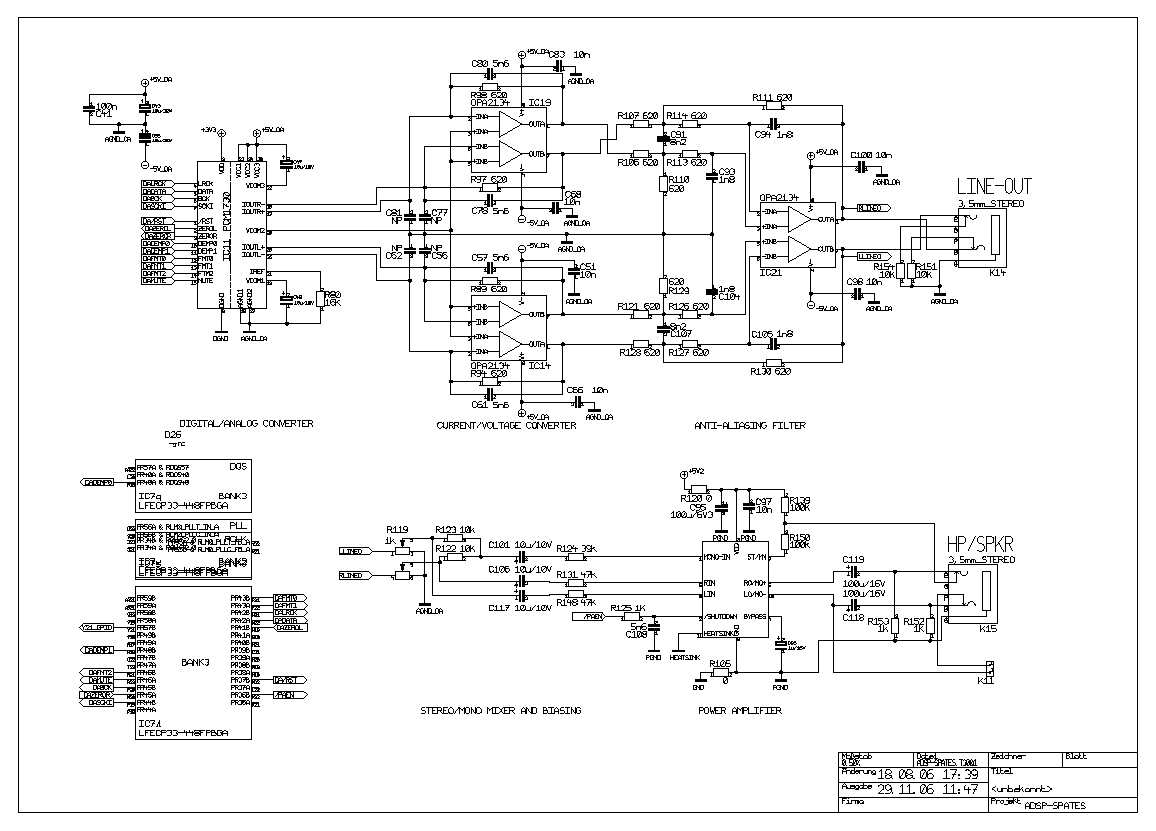
\includegraphics[angle=90,width=1.00\textwidth]{schematics/ADSP-SPATES_2}
%	\label{fig:schematic2}
%\end{figure}
%
%\begin{figure}[ht]
%	\centering
%		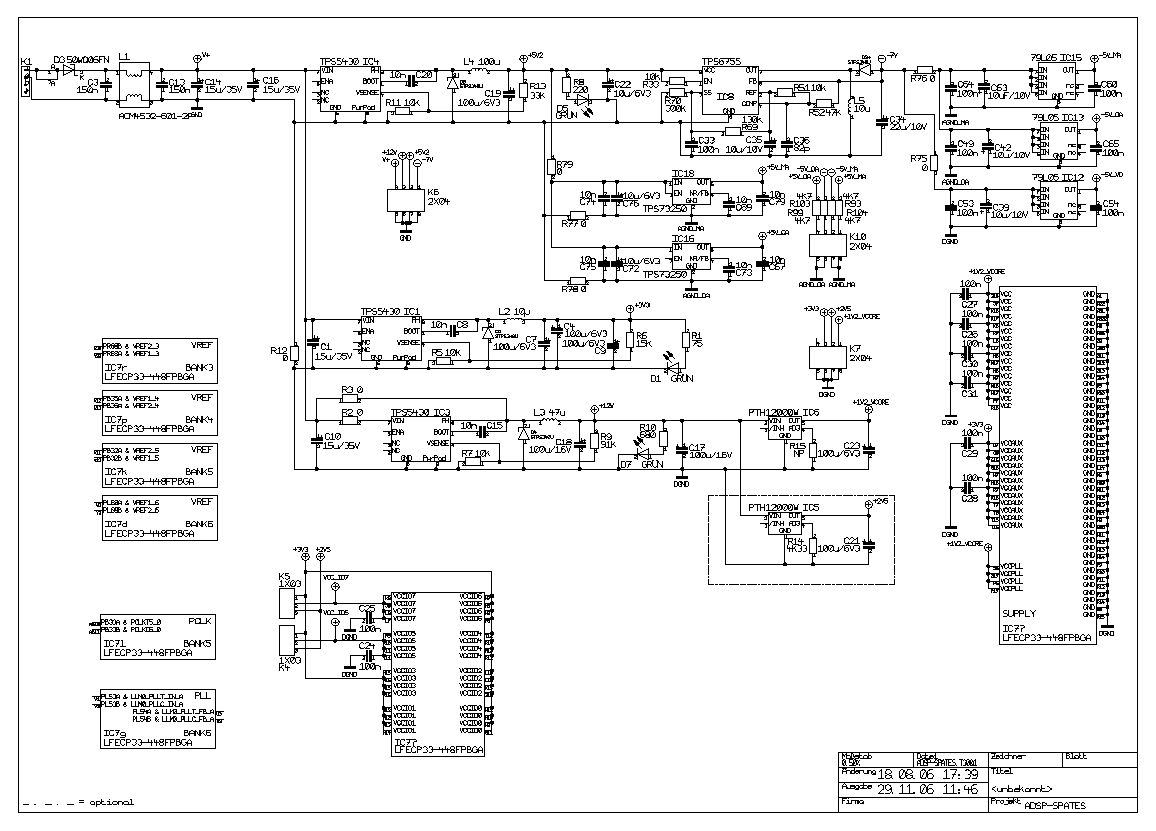
\includegraphics[angle=90,width=1.00\textwidth]{schematics/ADSP-SPATES_3}
%	\label{fig:schematic3}
%\end{figure}
%
%\begin{figure}[ht]
%	\centering
%		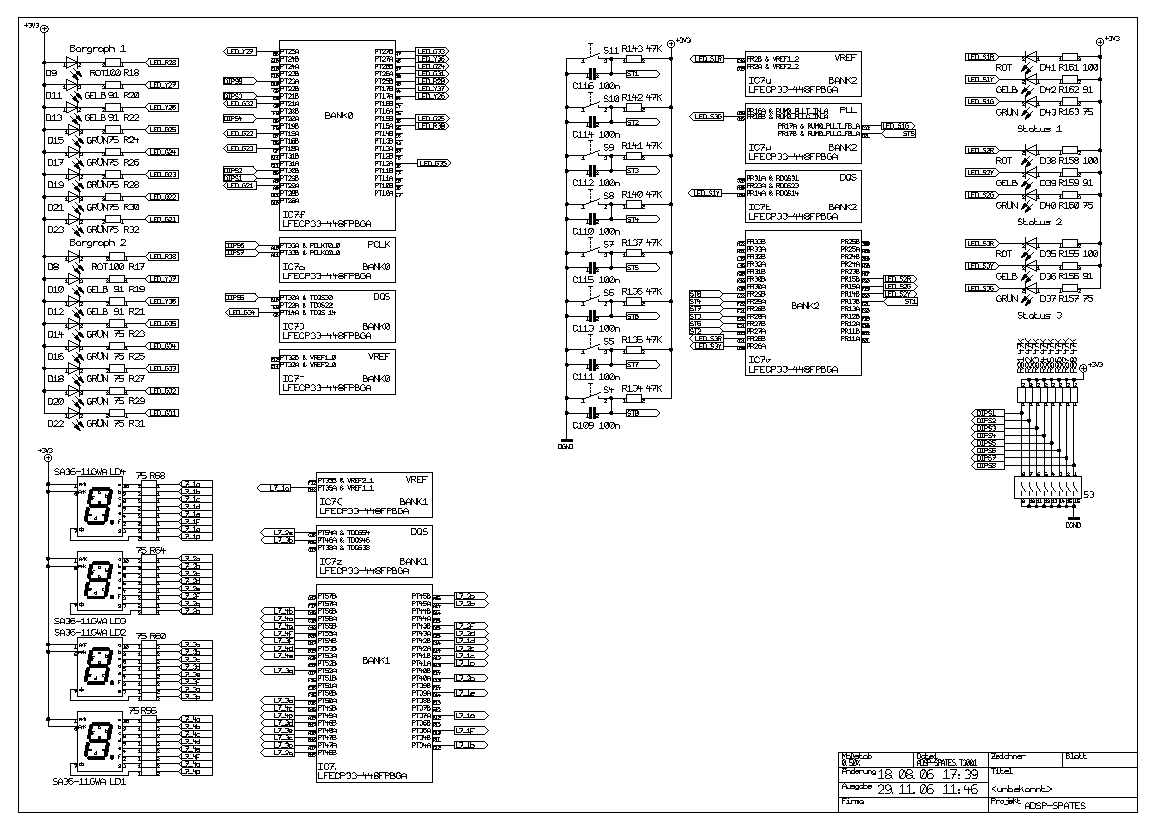
\includegraphics[angle=90,width=1.00\textwidth]{schematics/ADSP-SPATES_4}
%	\label{fig:schematic4}
%\end{figure}
%
%\begin{figure}[ht]
%	\centering
%		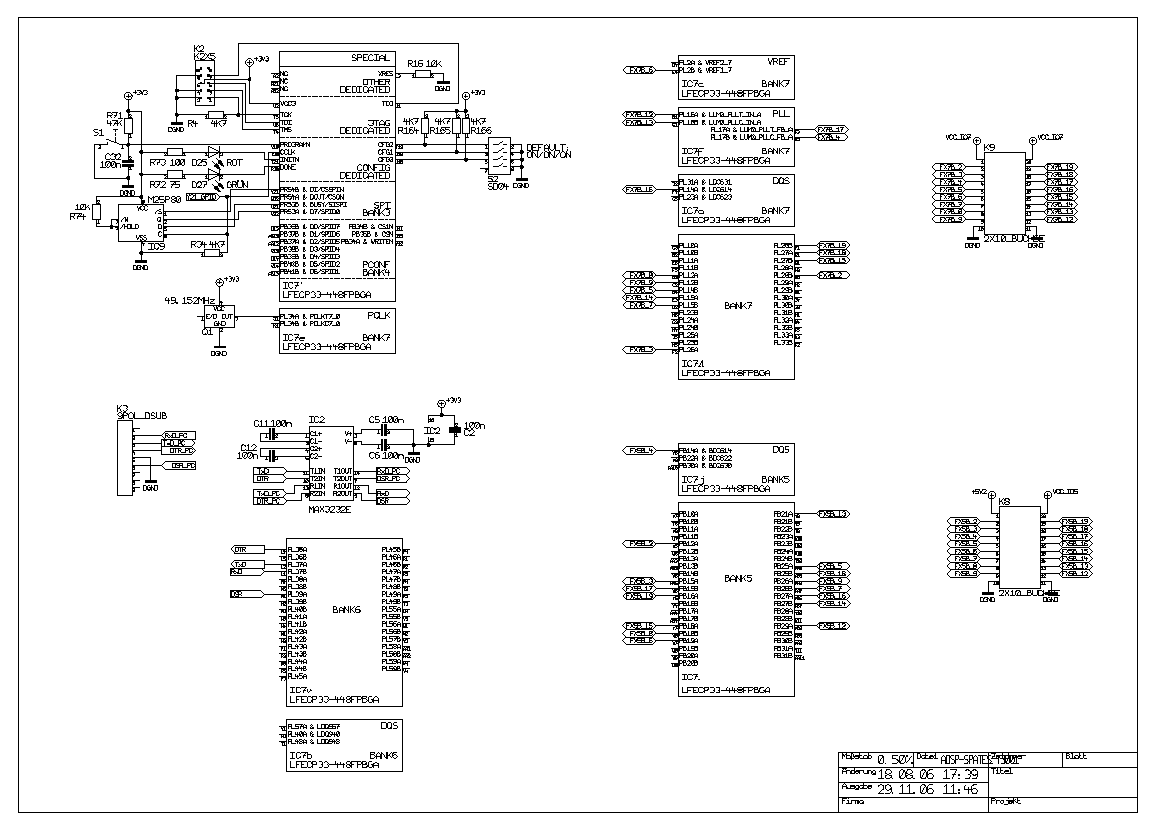
\includegraphics[angle=90,width=1.00\textwidth]{schematics/ADSP-SPATES_5}
%	\label{fig:schematic5}
%\end{figure}

\begin{center}

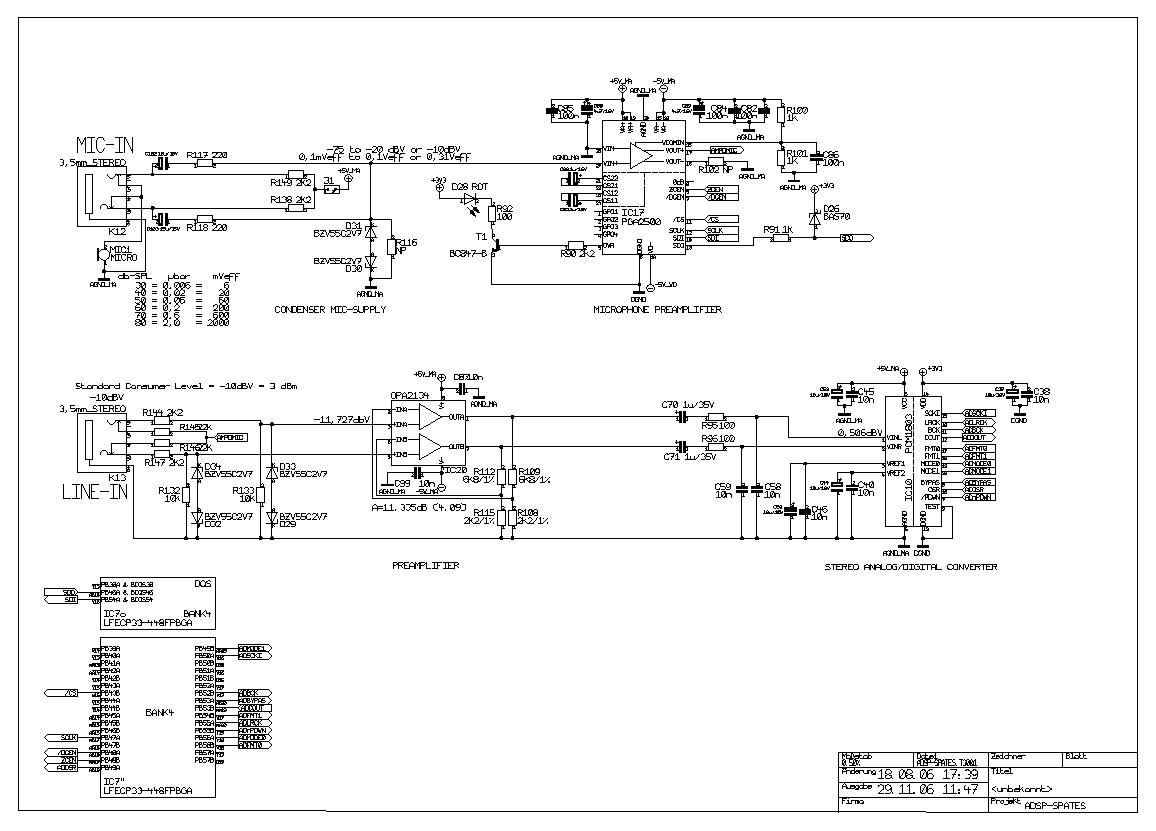
\includegraphics[angle=90,width=1.00\textwidth]{schematics/ADSP-SPATES_1}\label{fig:schematic1}

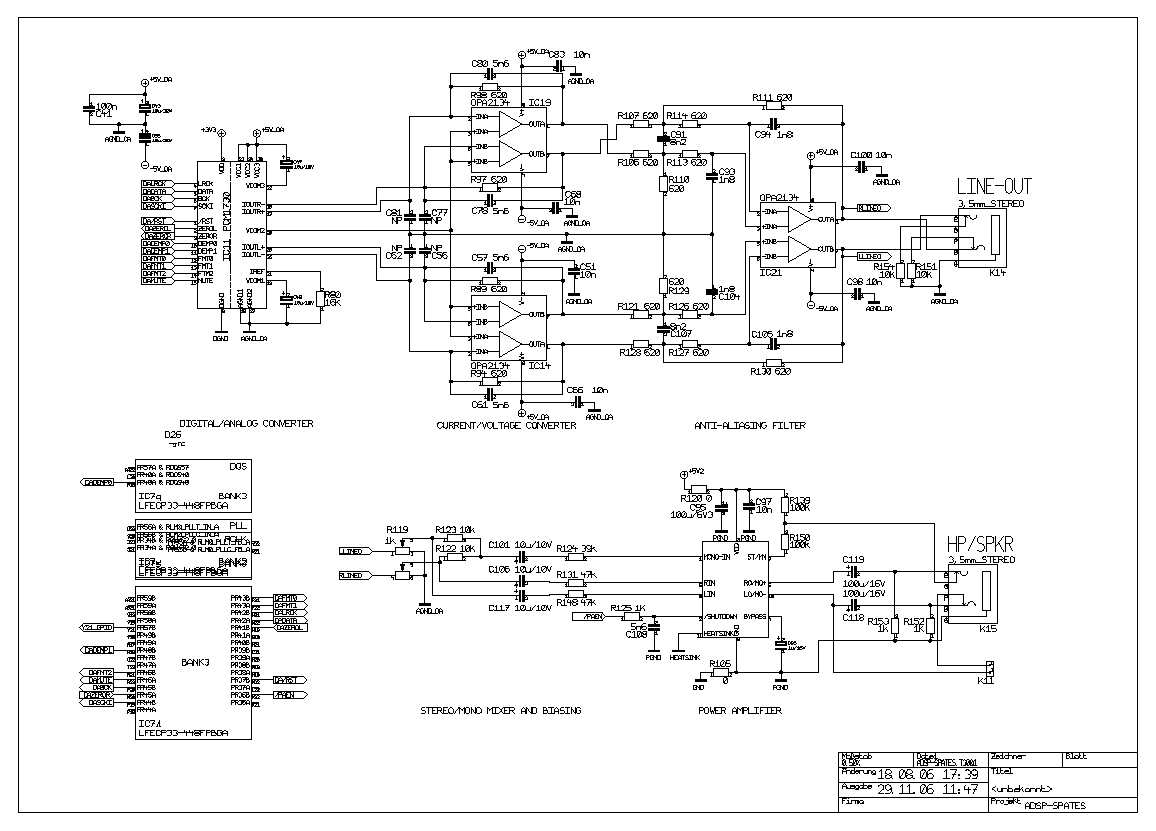
\includegraphics[angle=90,width=1.00\textwidth]{schematics/ADSP-SPATES_2}\label{fig:schematic2}

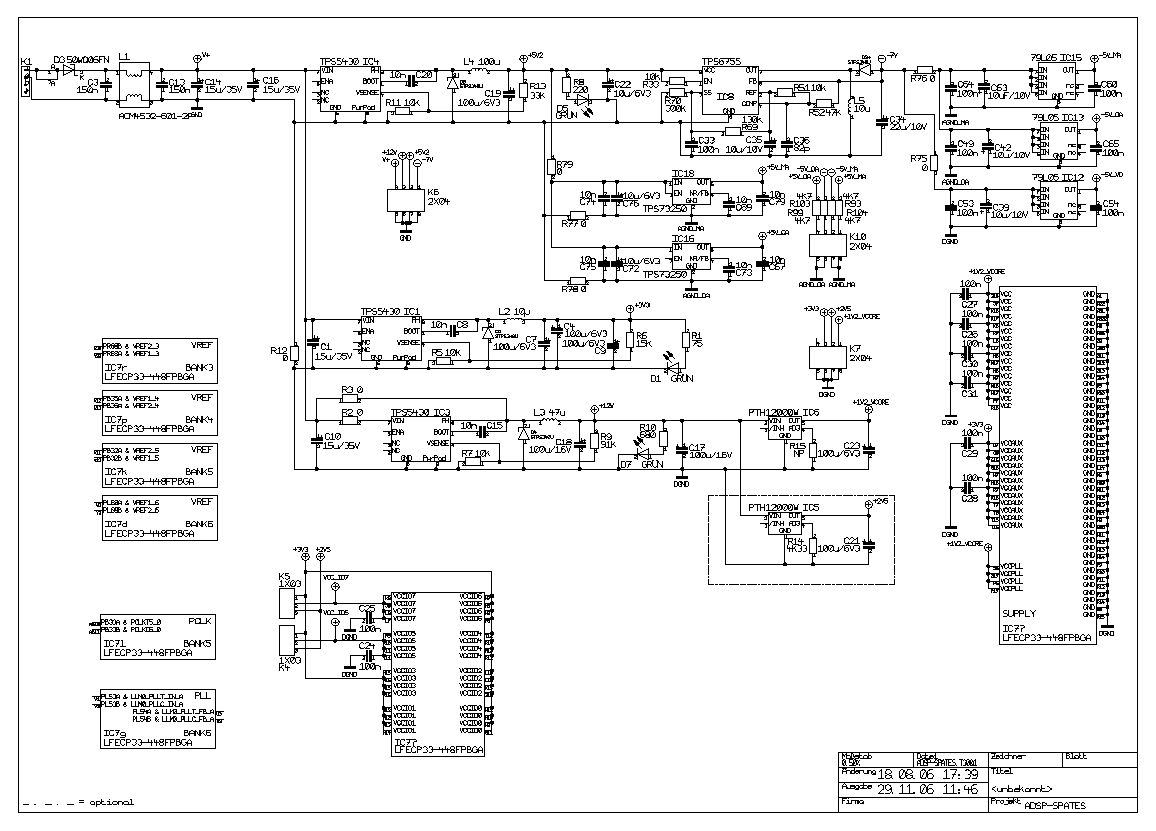
\includegraphics[angle=90,width=1.00\textwidth]{schematics/ADSP-SPATES_3}\label{fig:schematic3}

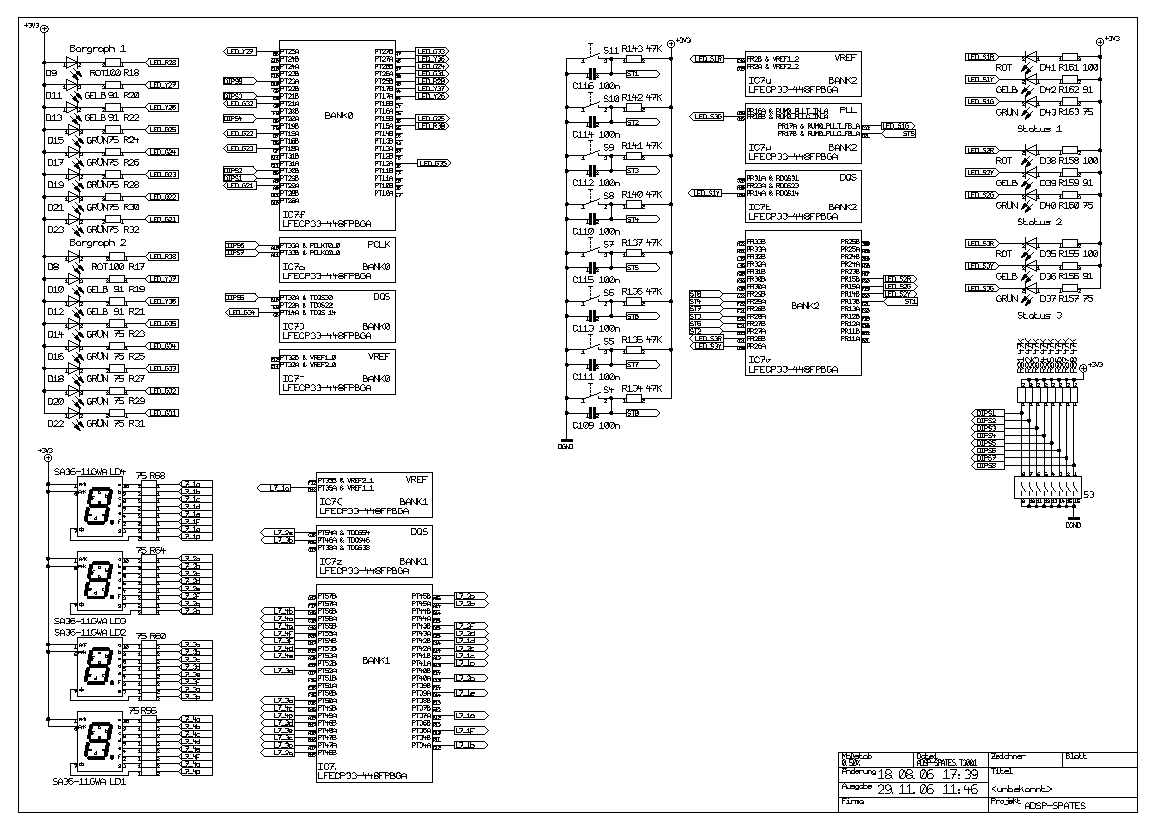
\includegraphics[angle=90,width=1.00\textwidth]{schematics/ADSP-SPATES_4}\label{fig:schematic4}

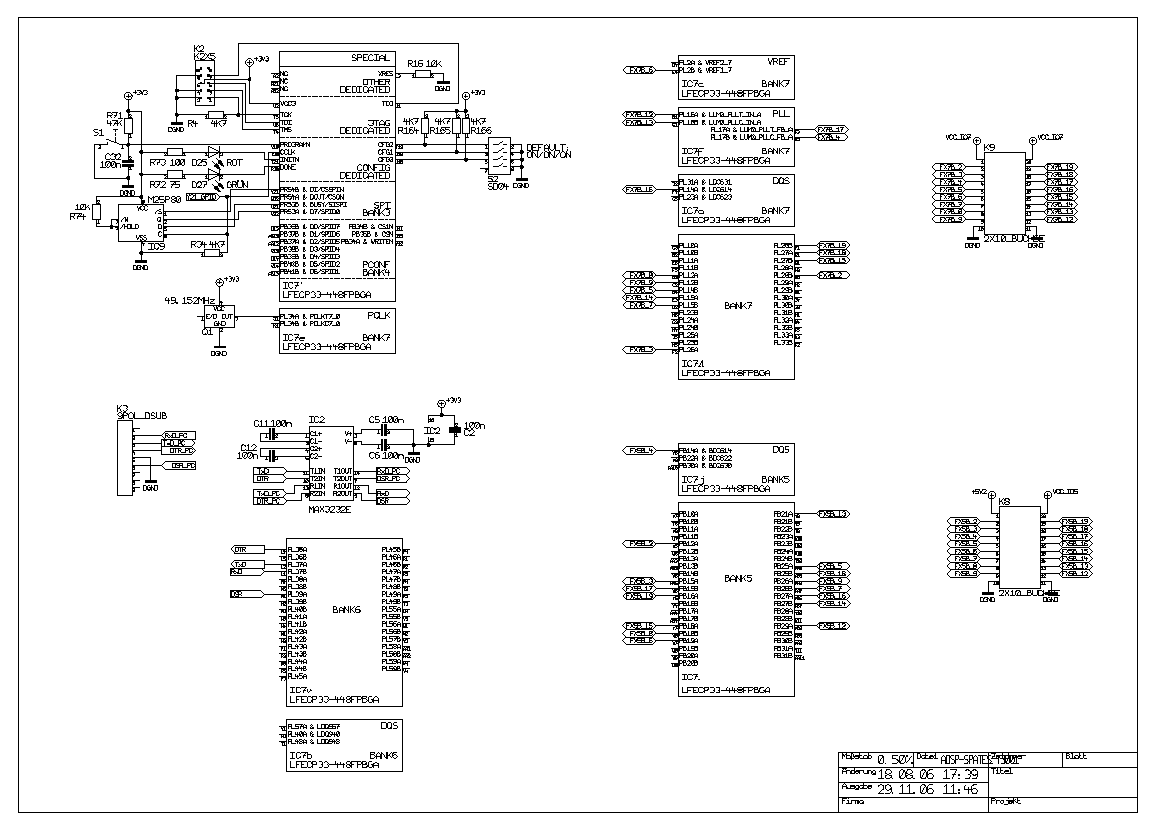
\includegraphics[angle=90,width=1.00\textwidth]{schematics/ADSP-SPATES_5}\label{fig:schematic5}

\end{center}


\section{Errata}

Folgenden Fehler und �nderungen sind bisher bekannt:

\begin{description}
	\item[C34] Polung falsch
	\item[C89] Polung falsch
	\item[R100] muss gegen +5V gehen
	\item[Q1] 32,768MHz wegen besserer Verf�gbarkeit
	\item[IC2] SP3232 anstatt MAX3232
\end{description}
